\documentclass[11pt]{beamer}
\usepackage{lmodern}
\usepackage{graphicx}
\usepackage{hyperref}
\usetheme{Singapore}
\author{Gerd Graßhoff}
\title{Algorithmische Geschichte und Philosophie der Wissenschaften, Vorl 4}
\date{9. Mai 2019}

\begin{document}
	\begin{frame}[plain]
		\maketitle
	\end{frame}


\section{Erkenntnisgewinn / Entdeckungsfeststellungen}

	\begin{frame}
	\frametitle{Wissenschaftstheoretische Schlüsselbegriffe}
	\begin{itemize}
		\item Forschungsobjekt / System / Planetensystem
		\item Modell
		\item Messungrozess / Instrument
		\item Data
		\item Befund / Ergebnis / Entdeckung / Erkenntnis
	\end{itemize}
\end{frame}

	\begin{frame}
	\frametitle{Ausdrücke der Entdeckung, Ergebnis, Fund}
	\begin{itemize}
		\item Entdeckung, neue Erkenntnis / Discovery, knowledge, finding
		\item Erforschung, Forschung / Research
		\item Detektion / detection
		\item Befund, Ergebnis / result
	\end{itemize}
\end{frame}

	\begin{frame}
	\frametitle{detect}
\begin{figure}
	\centering
	\includegraphics[width=0.7\linewidth]{screenshot001}
	\caption{Webster}
	\label{fig:screenshot001}
\end{figure}
\end{frame}

	\begin{frame}
	\frametitle{detect: Synonyme: Antonyme}
\begin{figure}
	\centering
	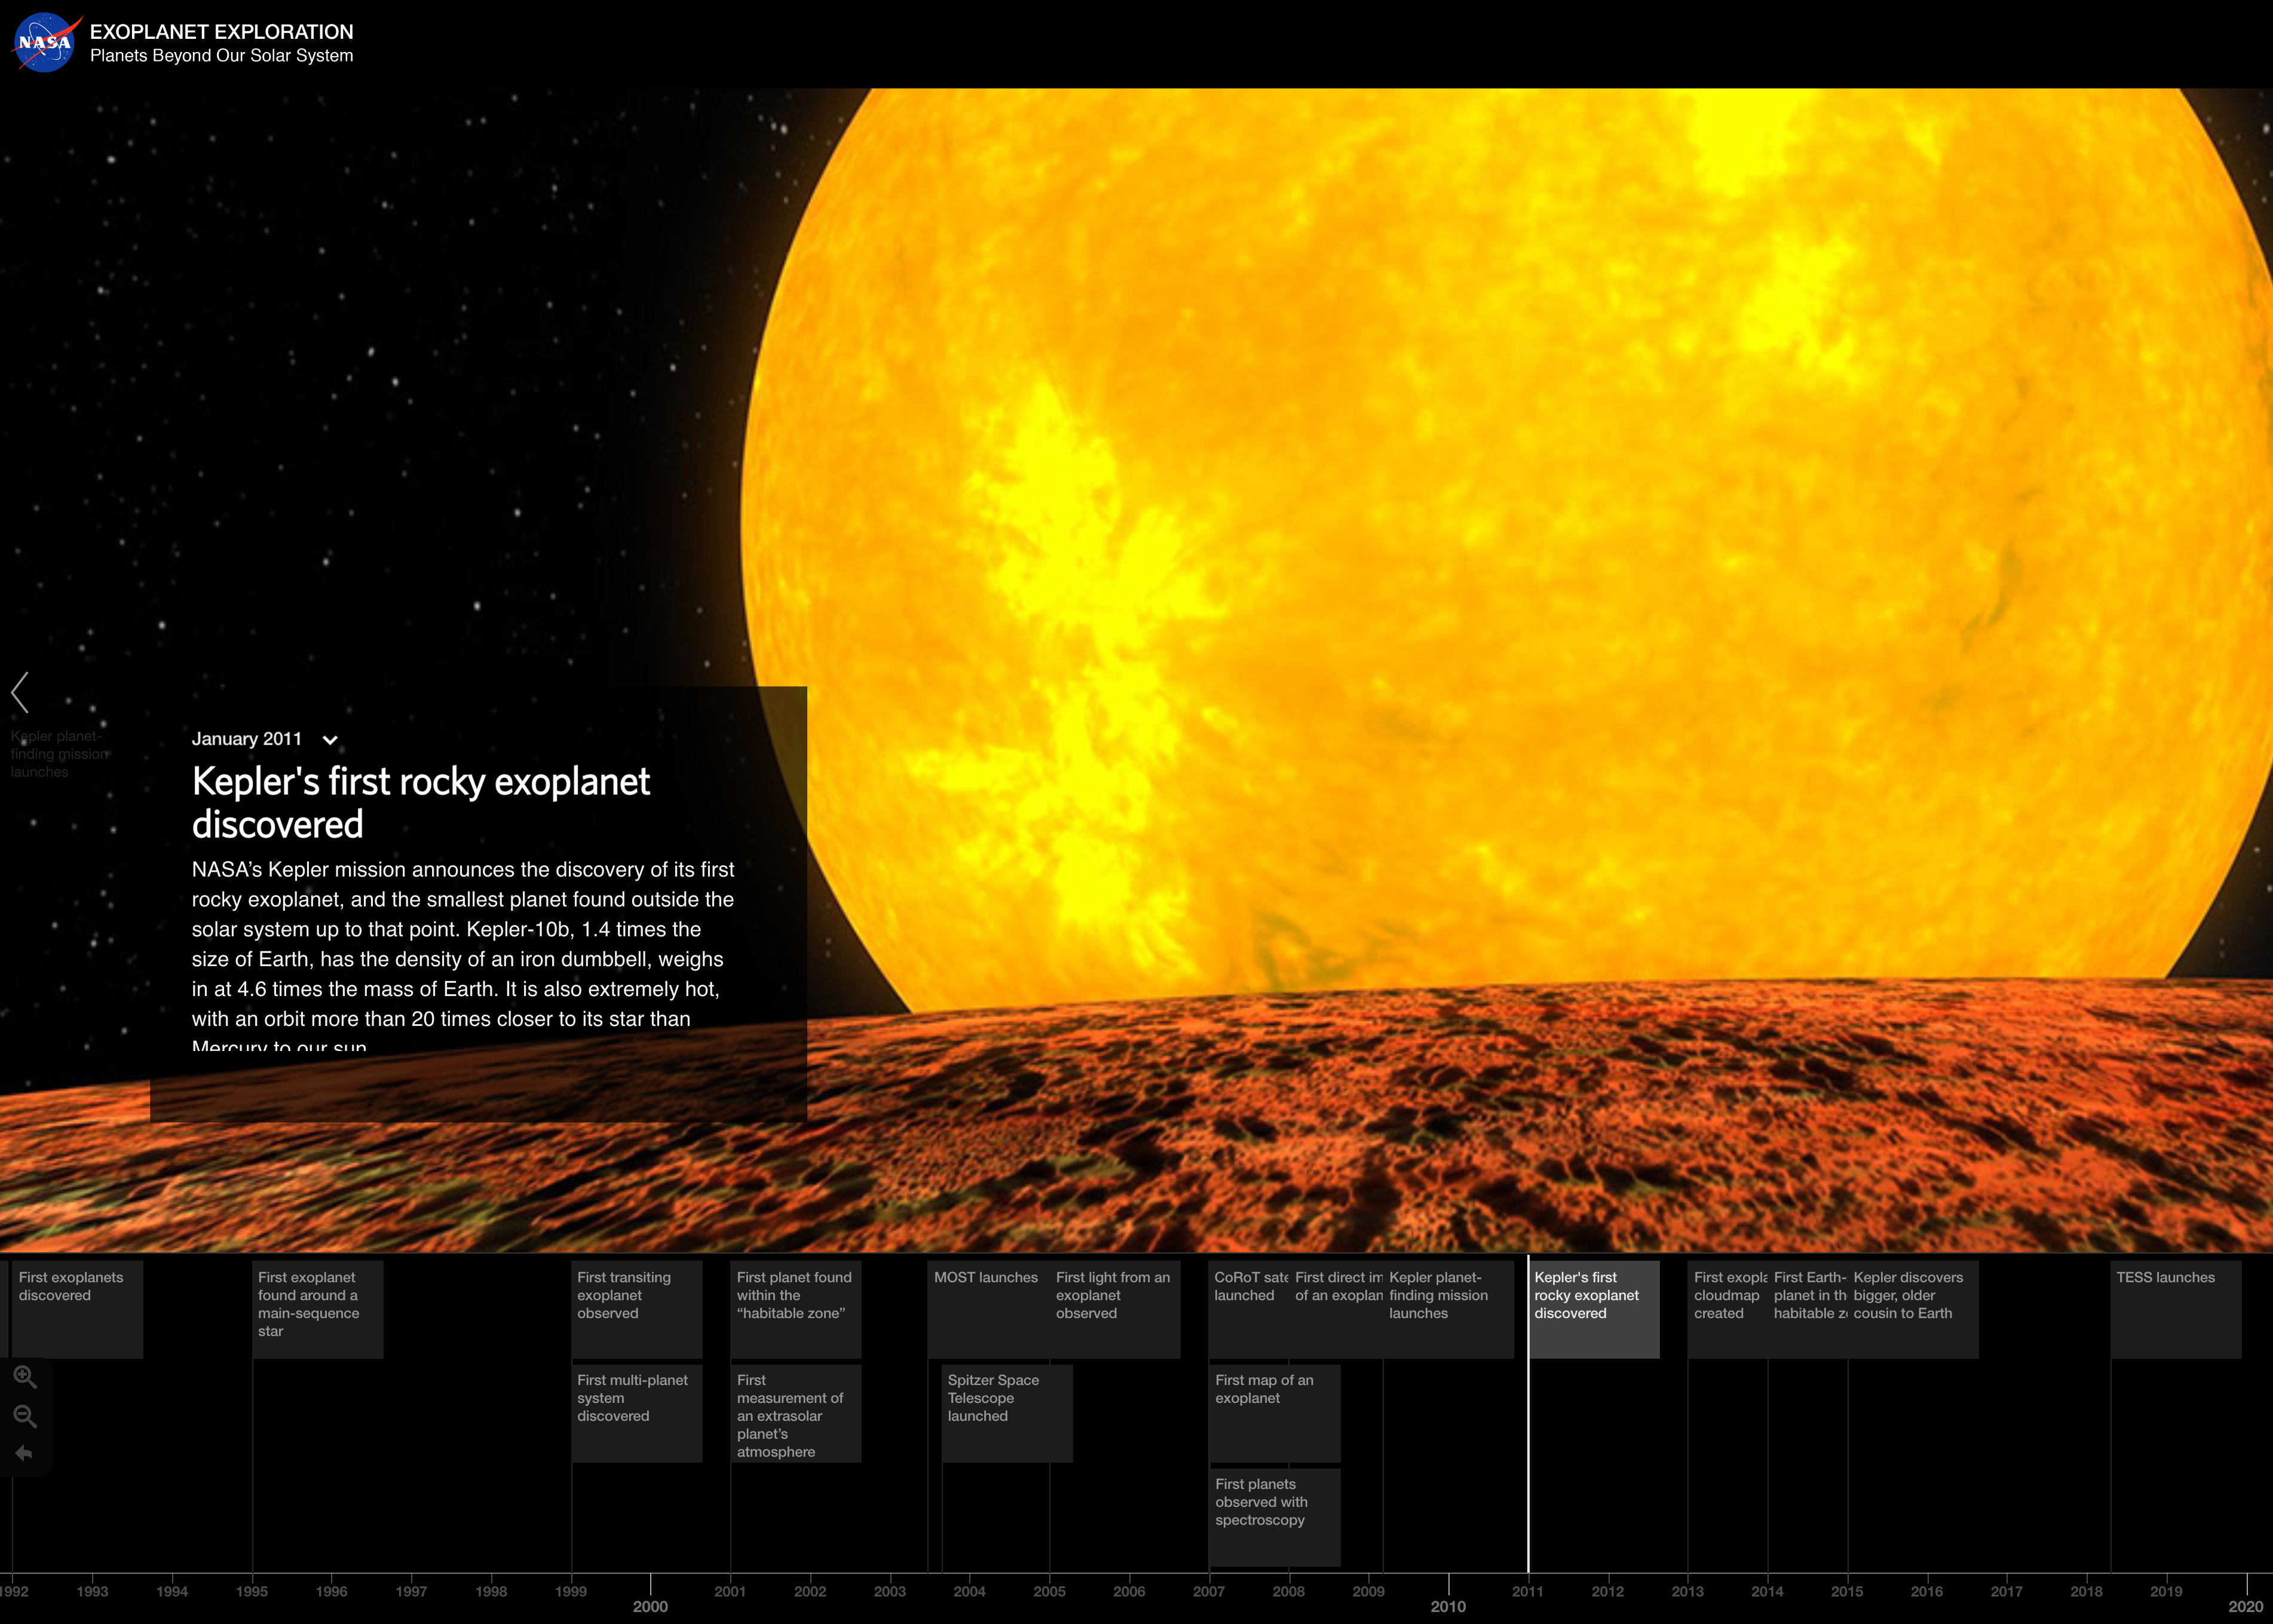
\includegraphics[width=0.7\linewidth]{screenshot002}
	\caption{}
	\label{fig:screenshot002}
\end{figure}
\end{frame}


	\begin{frame}
	\frametitle{Gründe einer Entdeckung: Rätsel der epistemischen Schlüsse!}
	\begin{itemize}
		\item Daten
		\item Messprozess / Instrument
		\item Modell
		\item Konklusion: Objekt x hat die Eigenschaft E: E(x)
	\end{itemize}
\end{frame}

	\begin{frame}
	\frametitle{Suche nach Erkenntnis: Rätsel der epistemischen Schlüsse!}
	Detection?: \href{https://iopscience.iop.org/article/10.3847/2041-8213/ab0e8d}{Detection}
	\begin{itemize}
		\item Daten O
		\item Messprozess / Instrument M -> O
		\item Modell Art(x) -> M(x)
		\item Konklusion?: Objekt x hat die Eigenschaft E: E(x)
	\end{itemize}
\end{frame}


\begin{frame}
	\frametitle{Messprozess}

	\begin{itemize}
		\item\href{https://exoplanets.nasa.gov/5-ways-to-find-a-planet/}{Messungen}
		\item\href{https://exoplanetarchive.ipac.caltech.edu/cgi-bin/TblView/nph-tblView?app=ExoTbls&config=planets}{Planetentabelle}
		\item\href{https://www.nasa.gov/mission_pages/kepler/overview/index.html}{Kepler Mission}
	\end{itemize}
\end{frame}

\begin{frame}
	\frametitle{Schlussform des Messprozesses}

	\begin{itemize}
	\end{itemize}
\end{frame}
sadf



\end{document}
